% \documentclass[a4paper,11pt]{report}
\documentclass[a4paper,11pt]{scrartcl}
\usepackage{setspace}
\usepackage[pdftex]{graphicx}
\usepackage[UKenglish]{babel}
\usepackage{url}
\usepackage{algorithmic}
\usepackage{rotating}

\pdfinfo {
	/Author (Asif Tamuri)
	/Title (Domain Network Graphs)
	/Subject (Biofinformatics visualization)
}

% Title Page
\title{Domain Network Graphs}
\author{Asif Tamuri
\\\\\\\\\\
\\\\\\\\\\
\\\\\\\\\\
\\\\\\\\\\
\\Supervisor: Roman Laskowski (EBI)
\\
\\School of Crystallography
\\Birkbeck, University of London
\\Malet Street
\\London WC1E 7HX}
\date {}

\begin{document}
\emergencystretch=11pt
\DeclareGraphicsExtensions{.jpg,.pdf,.mps,.png}
\maketitle
\thispagestyle{empty}

\doublespacing

\section*{Abstract}
\setcounter{page}{2}

\subsection*{Background}
% The abstract or summary should contain an outline of the work carried out and any significant results achieved. 
% \begin{itemize}
 % \item Is abstract between 200-300 words?
 % \item Does the abstract describe the nature of the work and the results obtained?
 % \item The abstract should contain key-words.
% \end{itemize}
% 
% The Abstract provides the reader with a summary of the contents of the dissertation. It should therefore be brief but contain sufficient detail, telling the reader the motivation for the work; project objectives; techniques employed; main results and conclusions. Abstracts should not normally exceed a page and should be self-contained.
% 
% The Abstract is the "gateway" to the contents of the dissertation, and therefore it is important that the Abstract gives the reader a good initial impression. Try to write Abstract with a "punchy" style.
% 
% (Write the Abstract last. The dissertation will be easier to summarise once all the bits are in place.)



Protein are annotated with domain and architecture information. However exploring the architecture landscape around a protein is currently challenging and there aren't any tools that allow bioinformaticians to visually browse and discover related proteins based on their domains and architectures. 

 

\subsection*{Results}
% Results go here
This paper presents DomVizApp and how it can be used to explore protein architectures. It is a desktop application which uses network graphs to visualise architecture similarities. The introduction describes the why domains and architectures are important, especially for discovering new drug targets. We then describe the data that was used along with the implementation of DomVizApp. We present the results of our data analysis and **"a case study is used to show how DomVizApp can help"** to explore architectures and discover new druggable proteins.
\subsection*{Conclusions}
% Conclusions go here
\thispagestyle{empty}
%\end{abstract}



\tableofcontents

% \section*{Acknowledgements}
%\addcontentsline{toc}{chapter}{\protect\numberline{}Acknowledgements}

 - 2,500 words for each section
%{{{ comments
% The introduction should record the background to the project and place the project in context with already published information. Essentially a literature review. It should also contain the aims of the project.
% 
 % \begin{itemize}
 % \item Discuss the motivation for the work that is being report
 % \item State and define the problem that the dissertation is trying to address or solve
 % \item State the aims and objectives of the work
 % \item Give an indication of how the work will be progressed
 % \item Provide a brief overview of each of the main chapters that the reader will encounter
 % \item Does the introduction contain a clear statement of the aims of the project?
 % \item Does the introduction place the project work in context with a thorough, but concise, review of the relevant literature.
 % \end{itemize}
 % 
 % What is the work trying to achieve and what you will be doing to meet these objectives.
 % 
 % (The objectives listed in this chapter will need to be achieved)
 % 
 % One of the last sections to write (i.e. based on the structure of the dissertation and the achieved contributions of the report -> enable you to state the objectives accordingly.)
 % 
 % \subsection{Literature Review}
 % 
 % The section is here for you to:
 % 
 % \begin{itemize}
 % \item Provide details about the motivation for the project.
 % \item State why the problem addressed by the dissertation is important.
 % \item Set the scene for the for the work
 % \item Describe what others have done and hence sets a benchmark for the current project
 % \item Justify the user of specific solution techniques or problem solving procedures.
 % \end{itemize}
%}}}


%{{{ introduction
\section{Introduction}
Find new drug targets and "Rationally score and assess the likely success of future drug targets."
"James Black is famously quoted as saying: 'the most fruitful basis for the discovery of a new drug is to start with an old drug'"

Drugs target a small number of targets and developing drugs against new families is slow. /cite{How many drug targets are there? - nature reviews}


The continuing growth, collection and annotation of protein data is leading to a requirement for tools to assist bioinformaticians to explore, analyse and discover relationships in these data. 

Protein domains and architectures are important annotations describing repeating motifs and units that are found repeatedly in multiple proteins. Proteins sharing domains or similar architectures have been shown to have similar or related function. It is possible to visualise architecture relationships and similarities by considering them as a network graph. These graphs assist users to views similar proteins that share domain architectures.

Graphs are often an ideal way of viewing biological data and there have been many areas of biology, such as metabolic pathways\cite{pathway_app} and protein interactions\cite{proteinint_app}, that have used network graphs and many tools are now available to visualise biological data (\cite{cytoscape}).

There have been much research to use networks or graphs to present and analyse protein domains and architectures. \cite{treeoflife}, \cite{proviz} However, there aren't any tools available that allow users to interact with and explore this data being presented visually. Most current solutions are one-dimensional lists and web pages which do not give a sufficiently broad view of protein relationships.
%}}}

%{{{ aim
\subsection{Aim} The work presented here describes the DomVizApp application, a new visualization tool to easily visualise, explore and locate proteins with similar architectures and domains. DomVizApp calculates similarity scores for architectures and uses these scores to render a graph which can be further filtered by users custom criteria. To be able to specify domains of interest; to see relatives of any protein chain and the domains that they have in common; the more common architectures are closer to the chain of interest; clearly see promiscuous domains compared with those domains that are less widely distributed (extremes); ultimately identify other proteins that have drug-binding domains; find related druggable proteins (defined as proteins with the same proteins architecture as drug targets) and druggable domains; 

We also present results of analysis of promiscuous domains and architectures.

We begin this introduction by describing protein domains and architectures and why they are important. We then review current techniques for measuring architecture similarity and finally discuss some of the tools available to explore proteins based on their domains and architectures.


%}}}

%{{{ protein domains and architectures
\subsection{Protein domains and architectures}
A protein domain is defined as ``a structural unit which can be found in multiple protein contexts'' \cite{pfamdb}. A `structural unit' usually refers to a subunit of the protein that can fold to a stable structure when separated from the globular protein. They are fundamental components present in the majority of proteins and they establish sequence or structural similarity for other proteins that share the same domain. Domains found in different proteins often share the same, or comparable, function. If proteins share several of the same domains, it can indicate that those proteins have a common, or related, function and may be evolutionarily related. It is known that the overall functions of two proteins related by jumbled domain architectures are often similar (The geometry of domain combination in proteins, Bashton M, Chothia, C).

A protein's domain architecture, or domain organisation, is the ``collection of domains that are present on a protein'' \cite{pfamdb}, and can be composed of one or more domains. Importantly, the architecture is the \textit{ordered} sequence of domains in a protein. Two proteins may share all the same domains but not share architectures due to a different order of domains. For example, an architecture with order of domains `XYZ' is not the same as the architecture `ZYX' even though they are composed of the same domains. Architectures link evolutionary related proteins \cite{fong} and proteins which share equivalent architectures can be loosely considered as homologous CITE-The geometry of domain combination in proteins, Bashton M, Chothia, C-CITE. Architectures can be used to group proteins rather than on sequence similarity. The combinations of domains into architectures give rise to the diversity we see in proteins. There has been much research into domain combinations and architectures and how they  lead to the particular function of a protein CITE-15,citation 16,17, pg2-CITE.   

REWRITE-Because of extensive analysis of domain architectures CITE-The geometry of domain combination in proteins, Bashton M, Chothia, C-CITE which show that protein with similar domains are homologs and more distantly related proteins will have different architectures, we can "infer" similarity of protein function and families by comparing their architectures.

There are several resources available for protein sequence domains. Pfam, SMART, CATH, PRODOM, SCOP. For DomVizApp we are using domain architectures from Pfam representing **fillme** sequences. Pfam is a large database of protein families and domains. Database of protein domains and families; represented by profile-HMMs; functional annotation of proteins; review current methods of searching for proteins with domains (i.e. web interface). The biological data is available as flat-files which have to be converted to a graph-based data structure for visualisation.
%}}}

%{{{ drug targets
\subsection{Drug targets} Drug development is an example of an area in which protein domains and architectures play an important role. A drug typically binds to a site on target. The targets are often recognisable domains on the protein (druggable domains); a drug that binds to a particular protein's domain is likely to bind to another related protein with the same domain (same family);

Identification of protein binding sites (3D)

Drug targets: ``Drug-target network'' Nature Biotechnology 2007 October Vol. 25 Num. 10; 
%}}}

%{{{ architecture similarity
\subsection{Architecture similarity}
Protein similarity is one of the most studied topics in bioinformatics. However, there is presently no canonical method to measure architecture similarity. Pfam score architecture similarity through a heuristic ranking \cite{pfam2002} of:
\begin{itemize}
	\item Number of domains in common, from identical domain architectures,
	\item Number of domains in common, through re-ordered combinations and
	\item Smaller number of common domains.
\end{itemize}

In addition to architectures sharing the same domains, architectures can also share domains that belong to the same clan, later introduced by  Pfam\cite{pfamdb}. Each clan contains domains that are thought to share a common evolutionary ancestor, which have been identified through:
\begin{itemize}
	\item Related structure,
	\item Related function,
	\item Substantial matches of sequences to HMMs for other families and
	\item HMM profile-profile comparison.
\end{itemize}

Each of these elements are used to score a relationship between domains. If the score is deemed significant, the domains are said to be in the same clan.

Other techniques for studying domain architectures include using the concept of fission and fusion of domains to build pathways of protein evolution \cite{fong}. A set of graph tools has also been developed to define the domain organisation of proteins in an entire organism \cite{cado}. The resulting graphs can then be used to compare different organisms. PRODOC \cite{prodoc} is a set of programs that enable comparison of proteins as a sequence of domains. These tools can be used to query the PRODOC dataset to identify proteins with a set of domains or the same domains but in a different order. 

Analysis of protein architectures: ``Modelling the evolution of Protein Domain Architectures Using Maximum Parsimony'' J Mol Biol. 2007 February 9; 366(1): 307-315; ``Comparative Analysis of Protein Domain Organization'' Genome Research 14:343-353;
%}}}

%{{{ visualisation
\subsection{Visualisation and its benefits}
Graphs are a common way to represent structured data with relationships within that data. The data is represented as nodes and relations are edges that connect the nodes. 

"Accurate visualisation of information allows users to quickly and effectively visualise importation features with groups."

"Graphs allow one to browse complex relationships and visualise key features of various grouping."

We use a sophisticated graph layout algorithm to render clear graphs with many nodes and complex relationships.

Pfamalyzer is a Java applet that allows users to explore Pfam architectures by querying the dataset using domains. The results are presented graphically in a ranked list.

\emph{Exploration of Pfam domain architectures:} ``PfamAlyzer: domain-centric homology search'' Bioinformatics Vol. 23 no 24 2007, pgs: 3382-3383.

%}}}


\section{Materials and Methods}

%{{{ comments 
%The materials and method section should describe in detail the procedures followed, indicating an awareness of any likely pitfalls or problems with the techniques. Published techniques need not be described in detail but should be referenced. The student should demonstrate an understanding of established techniques. \underline{N.B.} no results obtained by the student should appear in this section.
% 
% \begin{itemize}
 % \item Does this section describe in detail the procedures followed? Could you carry out this project following the methods reported here?
% \end{itemize}

% \begin{figure}[h]
	% \begin{center}
    % \includegraphics{es3d.pdf}
	% \end{center}
    % \caption{Example of an embedded pdf}
% \end{figure}
%}}}

%{{{ data sources 
\subsection{Data sources}
% WHERE THE DATA COME FROM
% WHAT THOSE DATA ARE
% FIGURE OF DATA SOURCES -> MYSQL DB WITH NAME OF SCRIPTS
% FIGURE OF DATABASE SCHEMA

The DomVizApp database was built by importing and linking the following sources: Pfam \cite{pfamdb}, Uniprot \cite{uniprot}, PDB \cite{pdb} and Drugbank \cite{drugbank}.

A collection of Perl modules were written to perform data pre-processing and to import the data into a MySQL\footnote{http://www.mysql.com/} database which acts as the master data store. These Perl scripts allow databases to be created given new data from Pfam, Uniprot or the PDB. Importing the data into a general purpose database allows us to easily integrate our data sources, facilitates flexible querying for analysis and allows for additional annotation in the future. The data sources, import scripts and database schema are illustrated in Figure~\ref{dataimport} and described below.  

\begin{figure}[h]
 \begin{center}
 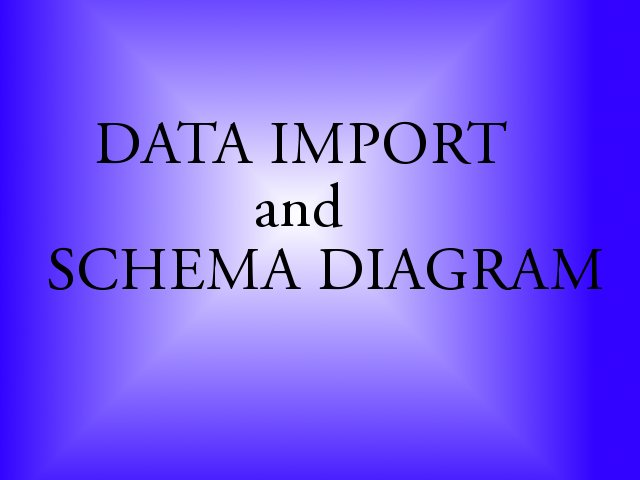
\includegraphics[scale=0.5]{figures/placeholder.jpg}
 \end{center}
 \caption{Overview of data sources and target schema}
 \label{dataimport}
\end{figure}

\subsubsection{Pfam}
Domains and architectures form the foundation of DomVizApp and were imported from Pfam version 22.0, available from the Pfam FTP site\footnote{ftp://ftp.sanger.ac.uk/pub/databases/Pfam/current\_release/swisspfam.gz}. The swisspfam dataset contains all the domains belonging to a sequence. Domains aren't presented linearly and the file requires additional parsing in order to extract the sequence's architecture. We extracted and loaded the sequence accession, Swissprot name and stored the sequence's architecture as a string with a dot-separated format (e.g. \texttt{D1.D2.D3.D1.D1}). The list of all Pfam clans (Pfam-C.gz) was also imported so that those domains that belonged to clans could be associated with other sibling domains. 

The dataset contains 45,684 distinct architectures (ignoring Pfam-B domains) from 9,318 domains, *fillme* of which are members of one of *fillme* clans.

\subsubsection{Uniprot}
In order to link domain architectures to sequences and taxonomy, Uniprot v14.0 (Swissprot 56.0) protein data were imported. The data includes all accession numbers for Swissprot entries, which allows us to link drug targets with Pfam sequence entries. We are also able to group sequences by identical domain organizations. This release contains 392,667 UniprotKB/Swissprot entries. % todo: only swissprot entries?

\subsubsection{PDB}
The PDB records were used to determine protein sequences that have had their structure solved. DomVizApp uses this information to allow users to filter for architectures that belong to a sequence that has had its structure determined. Links between PDB chain and Uniprot are only available in separate downloads for each individual chain from the Worldwide Protein Data Bank (wwPDB). Rather than downloading and parsing the full PDB database, we used the PDBSprotEC mappings \cite{pdbsprotec} which are available from the Bioinformatics Group at UCL\footnote{http://www.bioinf.org.uk/pdbsws/}. The dataset has 110,858 PDB chains mapped to *fillme* distinct Swissprot sequences. 

\subsubsection{DrugBank}
To analyse the targetting of proteins by drugs, details of drugs and their corresponding targets were obtained from the DrugBank \cite{drugbank} drugset as of 14 June 2008. The full drugcard set contains comprehensive drug data combined with drug-target data, such as sequence, Swissprot identifier and GO classification information. It also includes Pfam domains for each of the targets but it simply lists all the domains belonging to the target, not specifically the domains targetted by the drug. Only approved drug targets were considered in the analysis. The full drugcard set lists 4,764 drugs of which 1,484 are flagged as `Approved'. For our analysis, we only considered human targets. 

%}}}

%{{{ data analysis
\subsection{Domain architecture analysis}
% DESCRIBE ANALYSIS PERFORMED
% HOW THEY WERE PERFORMED
% WHY THEY WERE PERFORMED
After loading and integrating the different data sources, and having performed the necessary normalization of Pfam and Drugbank sequence accession numbers to the Uniprot primary accession number, we were able to perform some general analysis of the protein domain and architecture landscape. Using progressively selective criteria, we were able to retrieve summary information related to protein sequence Pfam entries, human protein domains and commonly occuring architectures.

For the first stage of analysis, a collection of SQL scripts were written to summarize the number of distinct domains and architectures and how frequently these domains and architectures occurred in sequences. We extracted this information for all species and HomoSapiens.

We also analysed the occurrences of domains in architectures, which required development of MySQL stored procedures as the information could not be retrieved using standard SQL set operations. We obtained these totals by getting a list of distinct domains and then iteratively searching for architectures that contained these domains. We retrieved total and HomoSapien numbers.

As mentioned previously, the purpose of this analysis was to survey the domain architecture landscape. As DomVizApp draws network graphs of related architectures, we wanted to have a sense of how large a typical graph would be (i.e. number of nodes) and what might be the worst case scenario. We were also able to see what types of domains were frequently occuring and investigate what was their related function.

The second stage of analysis was to investigate the possible number of `druggable' proteins in the human genome. Using the current DrugBank drug-target data we found the number of approved drugs currently targetting human proteins. We then retrieved additional protein sequences that had the same architecture as drug-targets but weren't currently targetted by any drugs.

To improve the number of probable druggable proteins, we should also include those sequences which have some of the domains (or all domains but in a different architecture) that specifically bind the drug. However, Drugbank does not currently state explicitly which domain the drug targets. We calculated the number of sequences that contain one or more of the same domains as the drug-target protein. This is likely to return an inflated figure of druggable targets as it is unlikely that a drug targets all the domains in a target protein.

This shortcoming is a reason that one of the goals of DomVizApp is to assist bioinformaticians to interactively explore protein architectures by allowing them to indicate domains of interest (say, a domain known to bind a drug) and then update the network graph accordingly.

%}}}

%{{{ implementation
\subsection{DomVizApp implementation}
% EVERYTHING THAT THE APPLICATION DOES AND USES
DomVizApp was wriiten in Java, using JDK 1.6. We used the Lucene search toolkit\footnote{http://lucene.apache.org/}, which was used to create high-performance search indexes of the biological data. The Prefuse toolkit \cite{prefuse}, a visualization framework for Java, was used to model graph data and visualize the network graph.

\subsubsection{Data preparation and indexing}
% Details of what the Lucene engine does for you and how exactly you used it for indexing your data
Our master data was stored in MySQL. As the schema was designed for data integrity and to reduce redundancy, its relational nature did not suit general-purpose querying. The performance of SQL queries was not fast enough to give DomVizApp users a highly interactive and dynamic experience. A common solution is to denormalise the data into new tables within MySQL that have been especially created for the types of queries that will be run against it.

As DomVizApp runs as a desktop application, we desired a solution that did not necessarily require the use of MySQL, which would require a database server to be installed and made accessible for the user. A better answer was to generate local, file-based, indexes that could be distributed to users of the application.

Lucene is a library for high-performance creation and searching of text indexes. By taking data from the master MySQL database and producing a Lucene index, we were able to have a separate, transferable, set of files that could be distributed to user's workstations. All the necessary information would be available locally to the user and this would facilitate the dynamic nature of DomVizApp.

The first stage was the indexing of our master data to create a searchable index. A Lucene index is stored as set of index files containing an inverted index data structure that allows rapid searching of text words. We interated through each sequence in Pfam, collecting data associated with it, such as its architecture and whether its structure has been solved, to create a Lucene \texttt{Document} which is a collection of fields. Each piece of Pfam data was stored as a field in the sequence Document.

We similarly created Documents for domain data, holding the Pfam domain identifier and its clan associations. 

Each of these documents was added to the Lucene index. The full workflow is shown in Figure~\ref{luceneworkflow}

\begin{figure}[h]
 \begin{center}
 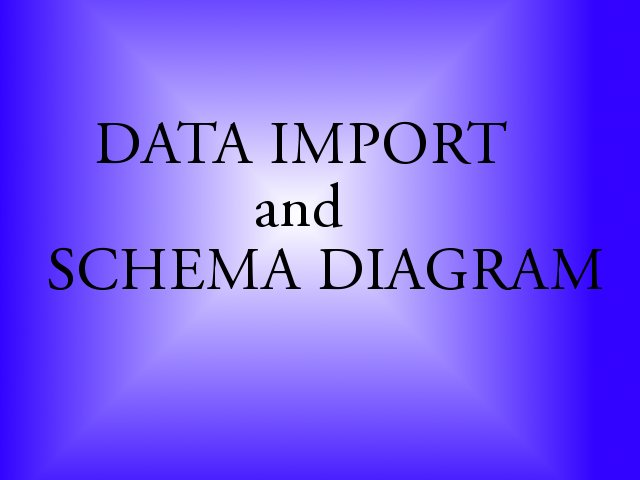
\includegraphics[scale=0.5]{figures/placeholder.jpg}
 \end{center}
 \caption{Lucene indexing workflow}
 \label{luceneworkflow}
\end{figure}

The Lucene index was searched from within DomVizApp based on user's specified criteria. Queries are written in a custom query language which is parsed by the Lucene index searcher. Lucene returns \texttt{Hits} matching the query and a reference to the original Document (e.g. Pfam sequence entry). We extracted the stored fields from these documents and were then able to use the data in DomVizApp.   

The total size of Lucene index was **fillme**Mb. Average query time to return data associated with a Pfam sequence was **fillme**ms and to return architectures containing a random domain took **fillme**ms on average. 

\subsubsection{Network graph visualisation}
% details of what the prefuse engine does for you and how exactly you used it for rendering network graphs. what is involved in customizing it for your application. a figure helps. show different components, highlight those that you need to customize/hack. describe layout techniques and force-directed layout in particular. what is the network graph meant to show
We are using network graphs to visually represent our data and their relationships. Graph visualisation is a fundamental component of DomVizApp and we used the Prefuse framework to both model graph data structures and to display the graph.

The framework provides interfaces and libraries for graph modelling, rendering and layout. Prefuse offers an API to control and customize almost all components of graph visualisation. The are several core components of the Prefuse framework, which are shown in Figure~\ref{prefuseframework} and described below.

\begin{figure}[h]
 \begin{center}
 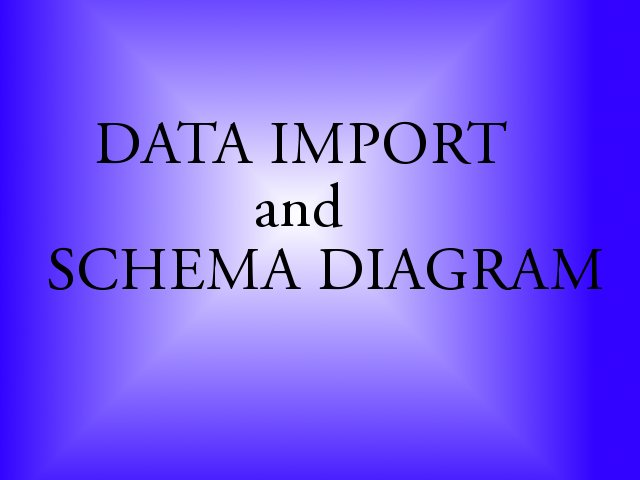
\includegraphics[scale=0.5]{figures/placeholder.jpg}
 \end{center}
 \caption{Components of the Prefuse Framework}
 \label{prefuseframework}
\end{figure}

\textbf{Data representation:} To model architectures and sequences we used the \texttt{Node} class. Their corresponding relationships were modelled using the \texttt{Edge} class. Both Node and Edge classes are subtypes of \texttt{Entity} which can hold any number of named elements with corresponding value. We stored Pfam domain identifiers, architectures, similarity scores and sequence names with their corresponding node or edge. This simplified querying of the graph itself as all biological data related to nodes or edges were stored with the entities themselves. No further lookup for data was required.

\textbf{Visual representation:} We then represented each node and edge as a \texttt{VisualItem}. A VisualItem stores the data related to entities and adds further properties related to the size, colour and other visual attributes. We used a different representation for architecture and sequences so they could be distinguished from each other.

\textbf{Interactions:} Prefuse \texttt{ActionLists} were used to respond to user actions and system events. These included executing the layout algorithm and adding callbacks to users clicking on nodes or edges. We were able to display the attributes of entities and collapse and expand sequence nodes in response.

\textbf{Rendering:} There are several algorithms provided for constructing network drawings and Prefuse allows most aspects of the layout algorithms to be customised. Due to the large number of nodes and edges, typical of bioinformatics datasets, standard graph rendering is tricky and usually not satisfactorily clear. We required not only a clear representation of the graph itself but also needed to be able to visualise features common to a group of architectures. DomVizApp uses a force-directed layout \cite{force}, provided by Prefuse, which attempts to place all the nodes by modelling entities as elements with physical forces that interact with each other. For example, edges have a spring force. All of these forces (gravity, spring and drag) can be customised as required. By simulating these forces across the nodes and edges, the layout brings connected nodes together and spreads unconnected nodes apart until the forces reach equilibrium, resulting in clear and expressive graphs. 

In DomVizApp, this means that two architectures that are similar will be placed closer in the resulting graph than architectures that are less similar. Groups of similar architectures will gather closer together. We customised the spring force of the edges which join architecture nodes and manipulated its properties based on the similarity score of the architectures. This modification brought architectures that are more similar than others closer together in the layout.

As this layout algorithm can be CPU-intensive, we allow the user to stop the the algorithm when a reasonable layout has been acheived. The final graph may not be mathematically the best graph but achieves an elegant layout \cite{force}.

\subsubsection{User interface}
% how it is laid out and what it requires to get started. what is the network graph meant to show
DomVizApp was designed to let bioinformaticians explore sequence architectures easily and clearly. The user interface was designed to encourage exploration through simplicity and responsiveness.

The interface is implemented using Java Swing libraries and the main screen is divided into 3-panes. The left pane is for user input: search, filtering and rendering options. The central pane displays the network graph. The bottom pane displays information about the current view or current user selection.

Users can interact with the graph pane using the mouse. The graph can be dragged, zoomed in or out and elements (nodes and edges) can be selected. Further information related to selected elements is displayed in the bottom pane.

To begin using DomVizApp, a user enters a protein sequence identifier. The application retrieves the architecture of the sequence (the `parent architecture'). It then searches for all architectures that share one or more domains with the parent architecture. These architectures, and sequences with these architectures, are visualised as a network graph. We allow the user to apply further filtering to this graph of results. For example, they may limit results to certain species or specific domains of interest. Because we are searching data held in an index stored locally, DomVizApp is able to quickly respond to changes in user's criteria and render new graphs.

The main component of the user interface is the network graph pane. Visualization of the similarity between architectures allows users to quickly and effectively interpret this information. Architectures and sequences are represented as nodes on the graph. All sequences are connected to their architecture by an edge. Architecture similarities are represented by an edge that connects architecture nodes to other architectures based on the strength of the similarity. We wrote rendering components for Prefuse to animate the addition and removal of nodes to highlight changes in the graph due to changes in criteria. 

%}}}

%{{{ computing architecture similarity
\subsection{Computing the scores for architecture similarity}

Given a set of architectures, all of which share a particular Pfam domain, one can obtain a matrix of all pairwise similarity scores between the architectures. We used such a matrix as the basis of the network graph to arrange architectures according to their relative similarities. We also used the similarity score to manipulate the spring forces for edges in the network graph to create clusters of similar architectures.

For DomVizApp, we used the Needleman-Wunsch algorithm \cite{nwalgo} to calculate this similarity score. The procedure is illustrated in Figure~\ref{computingscores} and described below. 

\begin{figure}[h]
 \begin{center}
 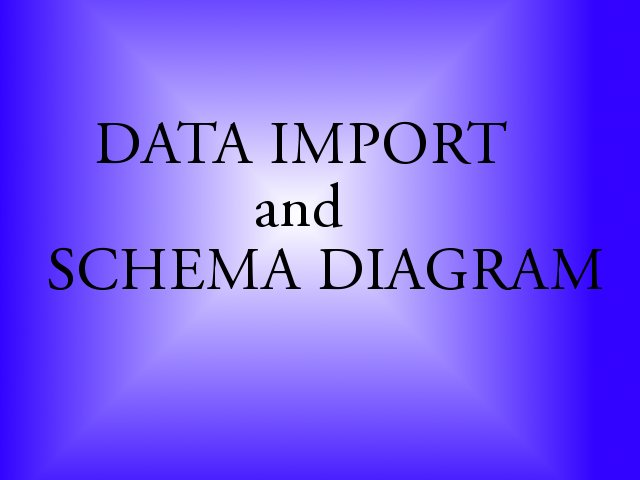
\includegraphics[scale=0.5]{figures/placeholder.jpg}
 \end{center}
 \caption{Calculating the all-against-all pairwise matrix of similarity scores}
 \label{computingscores}
\end{figure}

The first step in comparing any two architectures that share one or more domains was to create a similarity matrix scoring each of the domains present in the architectures. The score assigned to each pair in a similarity matrix may be simple, indicating a straighforward match or mismatch, or it may be related to a more sophisticated heuristic. For example, domain similarities could be measured using one of the techniques mentioned in the Introduction. The different heuristics and scoring techniques would ultimately result in different relationships among sets of architectures and therefore different graphs.

For the current version of DomVizApp, we used a scoring matrix that measures domain similarity based on:
\begin{enumerate}
	\item Domains matching exactly
	\item Domains belonging to the same clan, as defined by Pfam
	\item Domain mismatch
\end{enumerate}

Given the domain similarity matrix, we then used Needleman-Wunsch to perform an alignment of the two architectures based on their sequence of domains and obtain a maximal alignment score.

By applyting this technique for all pairs in a given set of architectures, an all-against-all pairwise matrix of similarity scores is calculated. 
%}}}

%{{{ using matrix of scores to draw network graph
\subsection{Using the matrix of scores to draw the graph}

To create the network graph, the calculated architecture similarity matrix was used to connect each architecture in the set with its highest scoring match. An edge was used to connect the two architecture nodes. 

To begin the process of connecting the architectures, we started with a graph of unconnected nodes. Each of the nodes represented an architecture in our set. First, we connected the parent architecture to its highest scoring match in the matrix. We then iterated over each of the unconnected architectures looking for the highest scoring match among the connected architectures. Once found, this unconnected architecture was joined to the connected architecture. We continued  iterating over unconnected architectures until all architectures had been connected to at least one other node.

If in the process of connecting architectures we found that there was an unconnected architecture which had the same high similarity score for two of more architectures, the architecture was connected to all of the high scoring architectures.
%}}}



\section{Results}

%COMMENTS:
	% Data must be presented in a form that makes clear the significance of any results obtained by the student. Wherever possible the results should be presented in the form of tables and graphs (with statistics where appropriate). You must also describe your results in the text. Attention should be drawn to interesting results but general discussion should be left until the next section. Figures should be used as appropriate.
	% 
	% \begin{itemize}
	% \item Does this section contain results in a tabular or graphical form?
	% \item Are the tables enumerated, each with a correct description of the contents? Are the columns and rows correctly labelled together with units of measurement?
	% \item Are the figures enumerated and appropriate for the type of data? Does each have a legend containing an accurate description of the contents of the figure?
	% \item Do graphs have axes labelled correctly (including units)? Is the scale of the axes appropriate for the data?
	% \item Are statistical results used when necessary? Are the correct tests used?
	% \item Are figures clearly labelled with a key to abbreviations in the legend and an accurate description of what they are?
	% \item Does the text draw attention of the salient features of the figures or tables, rather than simply repeat what is already in them?
	% \item Is the results section structured to make clear the significance of the results and to provide a basis for subsequent discussion?
	% \end{itemize}
	
	% Results: outcomes of all experiments.  For software, descriptions of the final system as well as initial systems.  Significant changes in direction should be documented and explained --- they are probably the result of something interesting you learned.  Description of a system includes an analysis of its performance (e.g. speed, domain of utility, usability).  
	
	% Do not try to maintain too rigid a distinction between Methods, Results, and Discussion. Someone reading your Results section will want to know why you did it, what you did, what the results are and what they mean - without having to flip backwards and forwards between other sections. There are no hard and fast rules here, and you may find after the first draft that some material is better in the Methods, or the Discussion, or vice versa. Some general guidelines are possible:
	% 
	% * the design of an experiment should be in the Results, and the details (usually) in the Methods
	% * if the details are necessary for understanding the results, that is where they should be - for example if you are comparing Southern blots at different stringencies, then the hybridisation and washing conditions must be in the Results. The legend to a figure or table is often a good place for this sort of detail.
	% * don't clog up the Results with unnecessary experimental detail
	% * preliminary experiments (e.g., developing and testing an assay) can go in either Methods or Results. But remember that the examiner may not read the Methods section in detail, so if you want her/him to be impressed by the amount of work you have done, or if you haven't got much else in the Results section, then put them into Results. But if you have a decent amount of results anyway, then putting less important stuff in can dilute the overall effect
	% * the best place to discuss what a result means is at the point when you are describing it. Don't feel that you have to hold it back for the Discussion, which would involve having to repeat chunks of your Results.
	% * if the interpretation of your results means having to refer to the literature, then it is probably better to do that in the Discussion. In general, we wouldn't expect many references in the Results section.
	% * the overall Golden Rule is to make it as easy as possible to read and understand
	% 
	% Your results section should not be a series of graphs and tables with no explanation  There should be:
	% 
	% * a short introduction to each section, explaining, briefly, the purpose and design of the experiment
	% * a reference to the results (either as Tables or Figures). All tables and figures must be numbered and each one must be referred to in the text. 
	% * a description which highlights the results that are of interest
	% * a description of how these results influenced the planning of the following results



\subsection{Domain and architecture analysis}
Uniprot chain; we get chain's architecture from Pfam; get related architectures (and chains) from Pfam; create nodes and edges;

\subsection{Visualization application}

\subsubsection{Graphs}
Graphs; different layouts? 

\subsubsection{Interaction}
Exploring the graph;


\subsection{Evaluation of architecture similarity}
Results of domain similarity across Pfam chains; (1,2...n domains in common); how will we evaluate whether our graphs are ``good''?


\subsubsection{Better techniques to generate similarity matrix}
Technique 2: Improved method based on domain phylogenetic tree paper
Let us also denote that the numbers of domain organizations of A and B are nA and nB, respectively, and the number of domain organizations shared by A and B is nAB. A and B initially share the same repertoires (i.e., nA = nAB = nB). As A and B diverge, nAB decreases because they independently accumulate new domain organizations and lose extant ones. Assuming that the gain and loss respectively follow the Poisson process, the evolutionary distance between O and A, dOA, is given by  dOA = -ln(nAB/nB)

Technique 3: Using profile-profile comparison tools such as PRC or HHsearch to create domain scoring matrix, then locally align domain architecture.

Technique 4: Use of Pfam clans - 2006

Technique 5: HMM-HMM comparison
influence of domain length; (design of custom algorithm?); strong vs weak similarity?

\subsection{How to know if graph is interesting graph?}
Technique for scoring architecture; does it have biological significance? e.g. are proteins with same/similar architecture involved in the same pathway?

\subsection{Data analysis}
Architecture searches: `and' vs `or' domain searches; for each domain, number of architectures; for each architecture, number of domains repeated in others (1,2..n times);

\subsection{Application: druggable domain discovery}
Application: druggable domain discovery

\subsection{Performance}
Number of nodes in graph; size of data set;



\section{Discussion}
% The discussion should examine in detail the significance of results and place them in the context of other published work. You should not reiterate your results. Any failings or shortcomings of the project should be identified. In this section consideration of the greater significance of the results should be demonstrated. An outline of what follow up work could be carried out may be useful (i.e. future work).
% 
% \begin{itemize}
 % \item Is it clear that the significance of the results is appreciated?
 % \item Are the results of the project discussed in relation to other published work in the field?
 % \item Are the results obtained discussed in the wider context?
 % \item Are the limitations of the approach used in this project adequately discussed?
 % \item Are any working hypotheses for future work proposed?
% \end{itemize}

\subsection{Analysis}
Comparing the top 10 promiscuous domains and architectures across all species against HomoSapiens show some "interesting differences".

\subsection{Comparison}
With other work in the field; discuss results in wider context;

\subsection{Limitations}
Failings and shortcomings;

\subsection{Extensions}
Future work and improvements;



%\renewcommand{\bibname}{References}                                                   
\addcontentsline{toc}{section}{\protect\numberline{}References}
\bibliography{references}
\bibliographystyle{jmb}

\clearpage

\appendix
\section*{Appendix}
\addcontentsline{toc}{section}{\protect\numberline{}Appendix}
\section{Example of Pfam source data}
\begin{verbatim}
>41_HUMAN         |====================| P11171.4 864 a.a.
4_1_CTD          1                 ---  (95) PF05902.4 4.1 protein C-terminal domain (CTD)  747-861
FA               1             --       (205) PF08736.2 FERM adjacent (FA)  498-544
FERM_C           1          ---         (410) PF09380.1 FERM C-terminal PH-like domain  405-494
FERM_M           1       ---            (757) PF00373.9 FERM central domain  292-401
FERM_N           1     --               (531) PF09379.1 FERM N-terminal domain  214-290
Pfam-B_153658    1 ---                  (2) PB153658   1-183
SAB              1                    --(78) PF04382.4 SAB domain  667-715
\end{verbatim}                    
\end{document}                           
                                 
                                 

